%============================
%User Management
%============================
\subsection{User Management}
This module is responsible for reading data from the client user database. It will do this by making use of ldap.js .
\subsubsection{Scope}
\paragraph{Test}
\subsubsection{Use cases}
\begin{itemize}
\item Autorize
\item validateUserName
\item retrieveEmail
\end{itemize}
\subsubsection{Domain model}

%============================
%Project
%============================
\subsection{Project}
The project module is responsible for the representation and persistence of all projects that the system will use to do the estimations on. This module will allow for complex projects to be created, as well as to be updated. A project is represented as a tree, consisting of a top-level project node and lower-level task nodes.

\subsubsection{Scope}

\subsubsection{Use cases}

\paragraph{Create a project - priority: critical}
Users with sufficient privileges can create projects.

\paragraph{Get project - priority: critical}
Users with sufficient privileges can retrieve projects to view them, or to be used for other purposes. This use case must thus return a representation of the project-tree, and not produce the output of the project tree.

\paragraph{Hide project}
\paragraph{Update project - priority: critical}


\subsubsection{Domain model}

%============================
%Estimation
%============================
\subsection{Estimation}
	The Estimation module will be responsible for handling all of the actions related to the estimation of a project. This involves allowing a user to place an estimate on a specific task as well as calculating the total estimation of a project.
\subsubsection{Scope}
	This is the estimation scope
	\begin{figure}[H]
	    	\centering
	    	\fbox{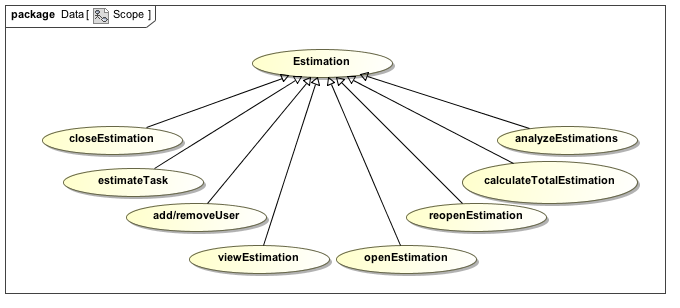
\includegraphics[width=0.5\textwidth]{Estimation_Scope}}
	    	\caption{Estimation Scope}
	    	\label{fig:Estimation_Scope}
   	\end{figure}
\subsubsection{Use cases}
	\paragraph{estimateTask - priority:critical}This system will allow a user to place an estimation on a task.
	\paragraph{calculateTotalEstimation - priority:critical}This system will traverse the project tree and calculate the total estimation of a project.
\subsubsection{Domain model}
\subsection{Report}
\subsubsection{Scope}
\subsubsection{Use cases}
\subsubsection{Domain model}
%============================
%Notification
%============================
\subsection{Notification}
This module will be responsible to notify all the users as required by the projects estimation. The estimation module will log a message request to the notification and add all the required users to notify.
\subsubsection{Scope}
This is the notification scope
	\begin{figure}[H]
	    	\centering
	    	\fbox{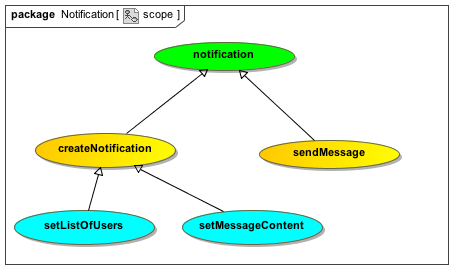
\includegraphics[width=0.8\textwidth]{Notification_Scope}}
	    	\caption{Notifications Scope}
	    	\label{fig:Notification_Scope}
   	\end{figure}
\subsubsection{Use cases}
The main purpose of notifications is to notify users with the required message. The estimation module will supply the list of users to notify and the contents of the message.
\paragraph{sendMesssage -- priority:mustHave}
\paragraph{createNotification -- priority:niceToHave}
\subsubsection{Domain model}
